\documentclass[journal]{IEEEtran}


\usepackage[pdftex]{graphicx}
\usepackage{amsmath}
\usepackage{multirow}
\usepackage{tabularray}
\usepackage{stfloats}
\usepackage[table,xcdraw]{xcolor}
\graphicspath{{../pdf/}{../jpeg/}}
\DeclareGraphicsExtensions{.pdf,.jpeg,.png}

% *** GRAPHICS RELATED PACKAGES ***
%
\ifCLASSINFOpdf
  % \usepackage[pdftex]{graphicx}
  % declare the path(s) where your graphic files are
  % \graphicspath{{../pdf/}{../jpeg/}}
  % and their extensions so you won't have to specify these with
  % every instance of \includegraphics
  % \DeclareGraphicsExtensions{.pdf,.jpeg,.png}
\else
  % or other class option (dvipsone, dvipdf, if not using dvips). graphicx
  % will default to the driver specified in the system graphics.cfg if no
  % driver is specified.
  % \usepackage[dvips]{graphicx}
  % declare the path(s) where your graphic files are
  % \graphicspath{{../eps/}}
  % and their extensions so you won't have to specify these with
  % every instance of \includegraphics
  % \DeclareGraphicsExtensions{.eps}
\fi


\hyphenation{op-tical net-works semi-conduc-tor}


\begin{document}
\bstctlcite{IEEEexample:BSTcontrol}

\title{Hybrid Improvement on Implicit Ranking Via BPR and WR-MF}

\author{MEHDI VALINEJAD,~\IEEEmembership{Student}}% <-this % stops a space

\markboth{Hybrid Improvement on Implicit Ranking Via BPR and WR-MF, VOL.~01, NO.~01, JANUARY~2024}%
{Shell \MakeLowercase{\textit{et al.}}: Hybrid Improvement on Bayesian Rank Prediction and WR-MF}

\maketitle

\begin{abstract}
To be completed
\end{abstract}

\begin{IEEEkeywords}
Hybrid Recommendation, Bayes Theorem, Bayesian Prediction, Item Based Recommendation System, Content Based Recommendation System, Weighted Ranking, Matrix Factorization, AUC, ROC.
\end{IEEEkeywords}

\IEEEpeerreviewmaketitle

\section{Introduction}

\IEEEPARstart{I}{tem} recommendation plays a pivotal role in delivering tailored content or products to users, anticipating their preferences and needs. 
The fundamental objective of this task is to predict a personalized ranking among a myriad of items, such as websites, movies, stocks, cryptocurrency or products. 
In this paper, I delve into a prevalent scenario where implicit feedback, including user actions like clicks, acquisition or purchases, guides the 
recommendation process.

Common approaches to item recommendation from implicit feedback, such as matrix factorization (MF) or adaptive k-nearest-neighbor (KNN), 
have been designed with the aim of personalized ranking. However, an intriguing observation surfaces: these methods, despite their 
intended purpose, are not directly optimized for the intricate task of ranking. In response to this gap, my research uses a set of
optimization criterion, termed BPR-Opt \cite{rendle2012bpr} and WR-MF \cite{8252119}, specifically tailored for personalized ranking. 
This criterion arises as the maximum posterior estimator derived from a Bayesian analysis of the problem.

In an effort to enhance the efficacy of BPR and WR-MF approach, I propose the incorporation of Content-Based analysis and ranking. 
This strategic addition aims to elevate the probability and evaluation metrics of BPR and WR-MF, further refining the accuracy and 
relevance of personalized recommendations. In the realm of content-based analysis, I aim to elevate the metrics of BPR and WR-MF 
through enhancements utilizing Jaccard, Cosine, Overlap Coefficient, Tversky Index and Dice Similarity. 

% === II. Literature Review ========================
% =================================================================================
\section{Literature Review}

Recommendation systems play a crucial role in sifting through vast amounts of information. Nevertheless, they frequently encounter 
challenges such as the cold start and sparsity problems, which hinder their overall effectiveness. Bayesian Personalized Ranking (BPR), 
designed to predict the relative order of user items, has traditionally been suggested to tackle these issues within ranking-based 
recommendation systems. However, conventional BPR methods heavily depend on implicit feedback and lack the inclusion of semantic 
and visual sentiment information. To bolster the efficacy of BPR, recent studies indicate that 
integrating diverse forms of side information, such as images, texts, videos, knowledge graphs, browsing history 
\cite{10.1145/3132847.3132941}\cite{8689028} and social network data, \cite{WU2024121930} can mitigate the sparsity inherent in the rating matrix. 

Employing a fusion of Convolutional Neural Networks (CNN) and Bayesian Personalized Ranking (BPR) presents a promising solution 
to tackle the cold start problem in friend recommendation systems (BayDNN) \cite{10.1145/3132847.3132941}. This innovative 
approach leverages the capabilities of deep neural networks to effectively handle scenarios where limited or no information is 
available for new users or items.

In response to the constraints of existing pairwise preference learning methods and "One-Class Collaborative Filtering", 
MSBPR \cite{ZENG2023110165} introduces a 
novel approach. Specifically, it addresses this limitation by formulating multi-pairwise preferences, achieved through a 
more detailed categorization of user non-interacted items into the user's potentially favored degree, the user's disliked 
degree, and the uncertain degree. This enhancement provides a more nuanced understanding of user preferences, contributing 
to the effectiveness of the MSBPR model.

Functioning as a content-based recommendation algorithm, Category-aided Multi-channel Bayesian Personalized Ranking (CMBPR) \cite{8689028} 
seamlessly integrates users' detailed preference data by considering variances across distinct video categories and various user interactions. 
Empirical results underscore the effectiveness of the CMBPR video recommendation algorithm, showcasing a significantly heightened level of 
recommendation accuracy in comparison to traditional video recommendation algorithms. Notably, CMBPR adeptly addresses the challenges posed 
by the "Long Tail" effect which is niche category short videos have the potential to expand and constitute a substantial proportion 
of the overall recommended short videos, providing a robust solution to enhance the quality of video recommendations.

To mitigate the sparsity challenges inherent in rating systems, the VBPR model \cite{Liang2020497} underwent optimization from various visual 
perspectives. This involved leveraging VGG features along with related visual attributes such as shape, color, and texture. 
Extracting visual features, including color and texture, from images was instrumental in enhancing the VBPR model. This 
optimization was built upon the foundation of the Matrix Factorization (MF) model.

In practice, the mere observation of items by users doesn't necessarily imply a preference for those items. Moreover, when 
dealing with the vast majority of items that go unobserved, it is oversimplified to categorize them as purely negative feedback. 
Mean Bayesian Personalized Ranking algorithm (MBPR) \cite{8946325} building upon the Bayesian Personalized Ranking (BPR) approach
categorizes observed interactions higher or lower than the average rating as positive or negative feedback and unobserved interactions 
are labeled with random values within a defined range. random assignment reflects the uncertainty about whether a user prefers 
unobserved items For each user, the interactions are categorized based on these criteria, offering a more nuanced and probabilistic
representation of user preferences compared to simplistic binary classifications.

The Listwise Bayesian Personalized Ranking (LBPR) \cite{He20171837} methodology is employed to calculate the likelihood of a ranking list for 
subsequent computation. Following the prediction of categories, Point-of-Interest (POI) candidates are filtered accordingly and 
ranked based on a dual strategy involving spatial influence and category ranking influence. This approach not only effectively 
tackles computational challenges but also enriches our comprehension of transition patterns between POIs. The outcome is a more 
robust and efficient next POI recommendation system within Location-Based Social Networks (LBSNs).

EBPRMF is employed for learning within each cluster, selecting Points-of-Interest (POIs) closest to the user's preferences to 
construct a recommendation list \cite{9296759}. This list is then presented to the user. Proposed as an improved iteration, EBPRMF refines 
the BPRMF recommendation algorithm by adjusting the POI similarity measurement, thereby augmenting its overall accuracy. 
Furthermore, to enhance recommendation diversity, this enhanced version introduces spectral clustering to the conventional 
BPRMF recommendation algorithm.

WR-MF \cite{he2017fast} enhances both the efficacy and efficiency of Matrix Factorization (MF) approaches in handling implicit feedback. We address two key 
challenges present in current methodologies. Firstly, many existing approaches tend to assign a uniform weight to unobserved 
feedback to mitigate computational complexity arising from the extensive space of unobserved data. However, this uniform 
assumption does not hold in real-world scenarios. Secondly, most methods are formulated in an offline context, lacking the 
adaptability required for the dynamic nature of online data. this method aims to tackle one-class collaborative filtering (OCCF) 
challenges through two distinct approaches: weighted low-rank approximation and negative example sampling which encompasses
assigning weights to the missing data according to the popularity of the items \cite{he2017fast}.

% === III. Methodology ========================
% =================================================================================
\section{Methodology}

To improve the performance metrics of Bayesian Personalized Ranking (BPR) and Weighted Regularized Matrix Factorization 
(WR-MF), a comprehensive formulation has been devised. This formulation is centered on extracting non-quantitative 
features from the content of items and leveraging them to establish similarity between items. The process involves 
selecting items with prior ratings for a specific user, considering them as potential items of interest related to 
the user's preferences. These selected items are then added to the list of highly ranked items for each user, thereby 
enhancing the recommendation system by incorporating both content-based and collaborative filtering approaches.
employing Category-aided Multi-channel Bayesian Personalized Ranking \cite{8689028} integrates multi-relational feedback sampling 
and category-aided sampling simultaneously to address this challenge. tourist attraction recommendation system, grounded in SS and 
enhanced VBPR, attained a commendable level of accuracy, effectively met user expectations, and significantly mitigated issues 
related to data sparsity.

\begin{figure}[!t]
  \centering
  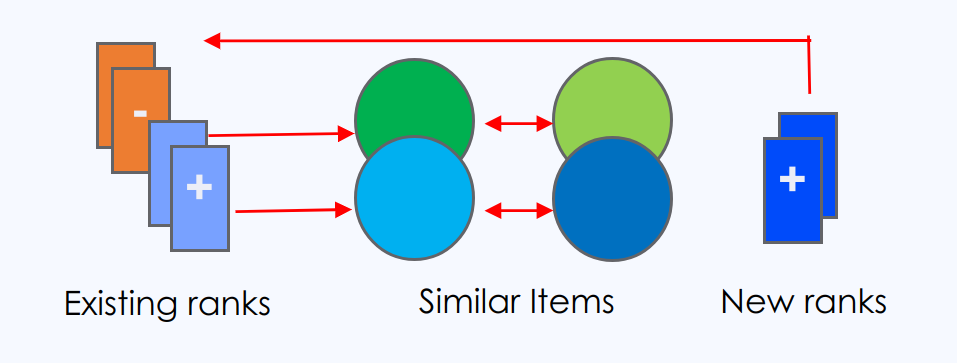
\includegraphics[width=3.5in]{picture/Novel-Ranks.png}
  By detecting positive rates corresponding items, novel rates will be added to the initial dataset. the similarity measure is
  responsible for matching similar items.
  \DeclareGraphicsExtensions.
  \caption{Simple loop of novel rate addition}
  \label{fig:novel_rate}
\end{figure}

\(Sims(I_i,I_j)\) computes the collection of akin items, given a minimum measured similarity threshold \(min_s\) that serves as the 
minimum acceptable similarity level between the items \(I_i\) and \(I_j\) This function is designed to generate a list of items 
that exhibit a degree of similarity equal to or greater than the specified minimum threshold, offering a comprehensive overview 
of related items in the context of their similarity to \(I_i\).

\[
  Sims(I_i, I_j) = \left\{ \begin{array}{ll}
    Sim(I_j,I_j) & \mbox{if $ \geq min_s$};\\
      & \mbox{if $ < min_s$}.\end{array} \right.
\]


\(Sim(I_i,I_j)\)  calculates the similarity between two items based on content-based metrics such as genre, tags, reviews, etc., 
utilizing Jaccard, Cosine, Overlap Coefficient \cite{953532}, Tversky Index and Dice similarity measures.

Given \(Sr(u_j)\) as the set of similar items for a particular user \(u_j\) with ranking higher than \(min_r\), 
the process involves computing the collection of movies that are similar to the user's top-rated movies (those with ratings
higher than \(min_r\)).
\[
  Sr(u_j) = \left\{ \begin{array}{ll}
    Sims(I_i,I_j) & \mbox{if $r_j \geq min_r$};\\
      & \mbox{if $r_j < min_r$}.\end{array} \right.
\]

Following the computation of the list of new ratings for each user, the next step involves appending these calculated 
ratings into the original rating array:
\[
N =
\begin{bmatrix}
  Sr(u_1)\\
  Sr(u_2)\\
  \vdots \\
  Sr(u_n)       
\end{bmatrix}
\]

Encompassing both the pre-existing ratings and the newly calculated ratings, \(N\) amalgamated array serves as a comprehensive 
repository of user preferences, capturing the dynamics of both historical and recently generated ratings. this will be used as
input variable to BPR and WR-MF algorithms for further and extended processing.

The methodology involves augmenting new ratings based on the similar items to those liked by each user. This process entails a 
random addition mechanism, where a shuffled list of users is employed to introduce new ratings for a specified number of items. 
Essentially, this approach involves updating the dataset with a pre-processed data before training the BPR and WR-MF models.

% === IV. Application ========================
% =================================================================================
\section{Application}

The hybrid model utilized the ml-1m dataset. Additional ratings were introduced into the rating data frame based on movies with 
similar genres, employing genre as the similarity measure. This was achieved by calculating the distance and filtering similar 
movies using mentioned similarity measures, with a threshold set at 0.9. The process involved iterating through each 
user's rankings and selecting movies with ranks exceeding 3.0 as positive feedback. This methodology essentially resembles 
implicit ranking, treating movies with ratings higher than 3.0 as though they have been watched.

Leveraging genres as a pivotal content medium, the extraction process involved meticulously curating a list of movies exhibiting a 
similarity threshold surpassing 0.9 for each user's set of rankings. Following this, a nuanced approach was implemented to append 
new ratings to these movies. The methodology for assigning these ratings was intricately tailored to align with the user's existing 
ranked values, drawing inspiration from the reference movie ranks.

This comprehensive procedure was systematically executed for the dataset comprising 1 million movies, ensuring a diverse representation 
across genres. To validate the robustness of the approach, the examination was extended to users randomly sampled for each movie. 
This iterative analysis provided a nuanced understanding of how user preferences and rankings were dynamically influenced by the 
intricate interplay of genres and similarity metrics within the dataset.

% === V. Results ========================
% =================================================================================
\section{Results}

\subsection*{1. Bayesian Personalized Ranking}

As an initial note, the Amazon Movies and TV shows review dataset was employed in the BPR implementation to evaluate the method's 
performance on other datasets with higher sparsity. The results indicate a lower AUC score, suggesting certain limitations in BPR's 
predictive capabilities when applied to real data with increased sparsity.

\begin{table}[htb]
  \resizebox{\columnwidth}{!}{%
  \begin{tabular}{|l|l|l|}
  \hline
  \textbf{AUC Score} & Train AUC & Test AUC \\ \hline
  Movielens\_1M      & 0.886287  & 0.852563 \\ \hline
  Movies\_and\_TV\_5 & 0.965592  & 0.773447 \\ \hline
  \end{tabular}%
  }
\end{table}

\begin{table*}[bp]
  \resizebox{\textwidth}{!}{%
  \begin{tabular}{|c|c|ccc|ccc|rrc|}
  \hline
                                                &                                & \multicolumn{3}{c|}{\textbf{AUC}}                                                                                   & \multicolumn{3}{c|}{\textbf{NDCG}}                                                       & \multicolumn{3}{c|}{\textbf{Recall}}                                                                                                      \\ \cline{3-11} 
  \multirow{-2}{*}{\textbf{Similarity Measure}} & \multirow{-2}{*}{\textbf{Set}} & \multicolumn{1}{c|}{\textbf{Prec1}} & \multicolumn{1}{c|}{\textbf{Prec2}} & \cellcolor[HTML]{F3F3F3}\textbf{Imp}    & \multicolumn{1}{c|}{\textbf{NDCG1}} & \multicolumn{1}{c|}{\textbf{NDCG2}} & \textbf{Imp} & \multicolumn{1}{l|}{\textbf{Recall1}} & \multicolumn{1}{l|}{\textbf{Recall2}} & \multicolumn{1}{l|}{\cellcolor[HTML]{F3F3F3}\textbf{imp}} \\ \hline
  \textit{Jaccard}                              & \textit{Test}                  & \multicolumn{1}{c|}{0.29687}        & \multicolumn{1}{c|}{0.35556}        & \cellcolor[HTML]{F3F3F3}\textbf{5.87\%} & \multicolumn{1}{c|}{0.33593}        & \multicolumn{1}{c|}{0.39632}        & 6.04\%       & \multicolumn{1}{r|}{0.13444}          & \multicolumn{1}{r|}{0.14473}          & \cellcolor[HTML]{F3F3F3}\textbf{1.03\%}                   \\ \hline
  \textit{Cosine}                               & \textit{Test}                  & \multicolumn{1}{c|}{0.29759}        & \multicolumn{1}{c|}{0.35748}        & \cellcolor[HTML]{F3F3F3}\textbf{5.99\%} & \multicolumn{1}{c|}{0.33655}        & \multicolumn{1}{c|}{0.39812}        & 6.16\%       & \multicolumn{1}{r|}{0.13396}          & \multicolumn{1}{r|}{0.143549}         & \cellcolor[HTML]{F3F3F3}\textbf{0.96\%}                   \\ \hline
  \textit{Overlap Coefficient}                  & \textit{Test}                  & \multicolumn{1}{c|}{0.29716}        & \multicolumn{1}{c|}{0.36228}        & \cellcolor[HTML]{F3F3F3}\textbf{6.51\%} & \multicolumn{1}{c|}{0.33703}        & \multicolumn{1}{c|}{0.40489}        & 6.79\%       & \multicolumn{1}{r|}{0.13561}          & \multicolumn{1}{r|}{0.14691}          & \cellcolor[HTML]{F3F3F3}\textbf{1.13\%}                   \\ \hline
  \cellcolor[HTML]{FFFFFF}\textit{TverskyIndex} & \textit{Test}                  & \multicolumn{1}{c|}{0.29814}        & \multicolumn{1}{c|}{0.35807}        & \cellcolor[HTML]{F3F3F3}\textbf{5.99\%} & \multicolumn{1}{c|}{0.33648}        & \multicolumn{1}{c|}{0.39856}        & 6.21\%       & \multicolumn{1}{r|}{0.13567}          & \multicolumn{1}{r|}{0.143}            & \cellcolor[HTML]{F3F3F3}\textbf{0.73\%}                   \\ \hline
  \textit{Dice}                                 & \textit{Test}                  & \multicolumn{1}{c|}{0.29688}        & \multicolumn{1}{c|}{0.35263}        & \cellcolor[HTML]{F3F3F3}\textbf{5.58\%} & \multicolumn{1}{c|}{0.33552}        & \multicolumn{1}{c|}{0.39056}        & 5.50\%       & \multicolumn{1}{r|}{0.13458}          & \multicolumn{1}{r|}{0.14028}          & \cellcolor[HTML]{F3F3F3}\textbf{0.57\%}                   \\ \hline
  \end{tabular}%
  }
  \caption{BPR results and metrics over train and test of ml-1m dataset}
  \label{table:bpr_scores}
\end{table*}

\begin{figure}[!t]
  \centering
  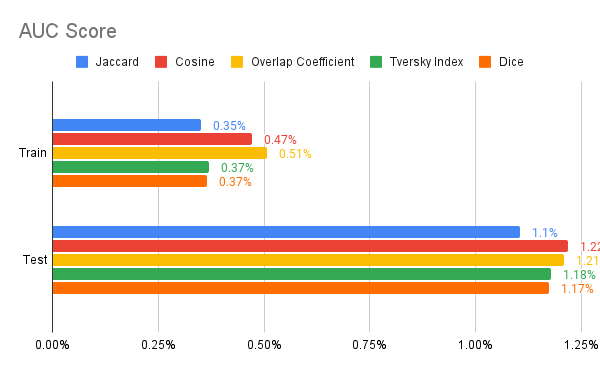
\includegraphics[width=3.5in]{picture/BPR-AUC-Score.png}
  For each similarity method, the chart values depict the percentage improvement achieved through the application of the respective 
  similarity measurement using BPR.
  \DeclareGraphicsExtensions.
  \caption{Improvement of AUC score after application of the hybrid method}
  \label{fig:bpr_auc}
  \end{figure}
  
  \begin{figure}[!t]
  \centering
  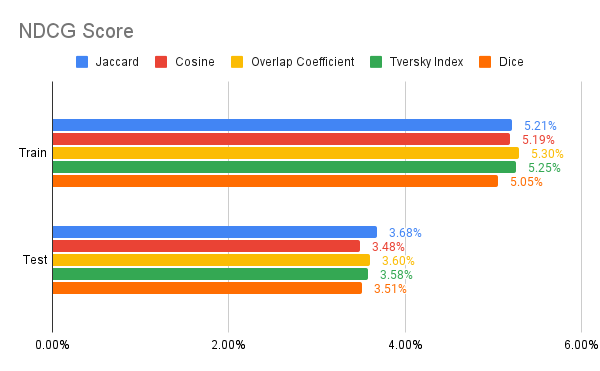
\includegraphics[width=3.5in]{picture/BPR-NDCG-Score.png}
  For each similarity method, the chart values depict the percentage improvement achieved through the application of the respective 
  similarity measurement using BPR.
  \DeclareGraphicsExtensions.
  \caption{Improvement of NDCG score after application of the hybrid method}
  \label{fig:bpr_ndcg}
  \end{figure}

Implemented the Bayesian personalized ranking \cite{rendle2012bpr} algorithm to forecast rankings using both the pure and extended ratings data frames. 
Employed the AUC Score metric as a benchmark study, serving as a pivotal measure for evaluating the prediction accuracy.

The updated rating data frame was supplied as input to BPR. The model was trained, and the AUC score of the predictions was 
computed. Consequently, the ensuing table presents the AUC scores corresponding to various sets of input combinations for  
\(Sr(u_j)\), aggregated across \(N\). This analysis provides a comprehensive overview of how different input configurations 
impact the AUC performance metrics.

The findings demonstrate a minor improvement, revealing a 0.51\% enhancement in the prediction AUC score for the training set and a 
noteworthy 1.21\% improvement for the test set when employing the Bayesian personalized ranking algorithm (BPR). 

Notably, these positive outcomes underscore the efficacy of the BPR algorithm in refining predictive performance. Moreover, 
the observed gains hint at the potential for even more remarkable results by augmenting the dataset with an increased number 
of novel ranks. As the number of ranks expands, there is a promising prospect of further refining the algorithm's ability 
to capture nuanced patterns and enhance its overall predictive accuracy.


Employing the aforementioned similarity measure to identify comparable items, the subsequent chart illustrates the enhancements 
observed in both the AUC score and NDCG score across both the training and testing datasets. The utilization of this similarity 
measure has evidently led to improvements in the predictive performance, as demonstrated by the notable shifts in AUC and NDCG 
scores in the chart depicted in Fig(\ref{fig:bpr_auc}) and Fig(\ref{fig:bpr_ndcg}). as evident from the observations, the Overlap 
coefficient and Cosine similarity measures exhibit superior performance in accurately matching similar items within the hybrid 
implementation. beyond the numerical scores, the AUC is revealed to be less reliant on the recently added ratings, making it a 
more robust method for predicting missing items.

\subsection*{2. Weighted Regularized Matrix Factorization}
The revised rating data frame served as the input for WR-MF. After training the model, the Precision, Recall, and NDCG for the 
predictions were calculated. Subsequently, the resulting table displays the Precision, Recall, and NDCG values associated with 
diverse input combinations for \(Sr(u_j)\), aggregated across \(N\). This examination offers a thorough understanding of how 
different input configurations influence not only AUC but also the Precision, Recall, and NDCG performance metrics.

\begin{table*}[htb]
  \resizebox{\textwidth}{!}{%
  \begin{tabular}{|c|c|ccc|ccc|}
  \hline
                                                                  &                                & \multicolumn{3}{c|}{\textbf{AUC}}                                                                                 & \multicolumn{3}{c|}{\textbf{NDCG}}                                                                                  \\ \cline{3-8} 
  \multirow{-2}{*}{\textbf{Similarity Measure}}                   & \multirow{-2}{*}{\textbf{Set}} & \multicolumn{1}{c|}{\textbf{AUC1}} & \multicolumn{1}{c|}{\textbf{AUC2}} & \cellcolor[HTML]{F3F3F3}\textbf{Imp}    & \multicolumn{1}{c|}{\textbf{NDCG1}} & \multicolumn{1}{c|}{\textbf{NDCG2}} & \cellcolor[HTML]{F3F3F3}\textbf{Imp}    \\ \hline
                                                                  & \textit{Train}                 & \multicolumn{1}{c|}{0.886071}      & \multicolumn{1}{c|}{0.889586}      & \cellcolor[HTML]{F3F3F3}\textbf{0.35\%} & \multicolumn{1}{c|}{0.532628}       & \multicolumn{1}{c|}{0.584745}       & \cellcolor[HTML]{F3F3F3}\textbf{5.21\%} \\ \cline{2-8} 
  \multirow{-2}{*}{\textit{Jaccard}}                              & \textit{Test}                  & \multicolumn{1}{c|}{0.85208}       & \multicolumn{1}{c|}{0.863133}      & \cellcolor[HTML]{F3F3F3}\textbf{1.1\%}  & \multicolumn{1}{c|}{0.340224}       & \multicolumn{1}{c|}{0.377007}       & \cellcolor[HTML]{F3F3F3}\textbf{3.68\%} \\ \hline
                                                                  & \textit{Train}                 & \multicolumn{1}{c|}{0.885419}      & \multicolumn{1}{c|}{0.890127}      & \cellcolor[HTML]{F3F3F3}\textbf{0.47\%} & \multicolumn{1}{c|}{0.534402}       & \multicolumn{1}{c|}{0.586267}       & \cellcolor[HTML]{F3F3F3}\textbf{5.19\%} \\ \cline{2-8} 
  \multirow{-2}{*}{\textit{Cosine}}                               & \textit{Test}                  & \multicolumn{1}{c|}{0.851683}      & \multicolumn{1}{c|}{0.863857}      & \cellcolor[HTML]{F3F3F3}\textbf{1.22\%} & \multicolumn{1}{c|}{0.342056}       & \multicolumn{1}{c|}{0.376879}       & \cellcolor[HTML]{F3F3F3}\textbf{3.48\%} \\ \hline
                                                                  & \textit{Train}                 & \multicolumn{1}{c|}{0.886287}      & \multicolumn{1}{c|}{0.891349}      & \cellcolor[HTML]{F3F3F3}\textbf{0.51\%} & \multicolumn{1}{c|}{0.534955}       & \multicolumn{1}{c|}{0.587915}       & \cellcolor[HTML]{F3F3F3}\textbf{5.30\%} \\ \cline{2-8} 
  \multirow{-2}{*}{\textit{Overlap Coefficent}}                   & \textit{Test}                  & \multicolumn{1}{c|}{0.852563}      & \multicolumn{1}{c|}{0.864642}      & \cellcolor[HTML]{F3F3F3}\textbf{1.21\%} & \multicolumn{1}{c|}{0.342198}       & \multicolumn{1}{c|}{0.378239}       & \cellcolor[HTML]{F3F3F3}\textbf{3.60\%} \\ \hline
  \cellcolor[HTML]{FFFFFF}                                        & \textit{Train}                 & \multicolumn{1}{c|}{0.886051}      & \multicolumn{1}{c|}{0.889753}      & \cellcolor[HTML]{F3F3F3}\textbf{0.37\%} & \multicolumn{1}{c|}{0.534571}       & \multicolumn{1}{c|}{0.587118}       & \cellcolor[HTML]{F3F3F3}\textbf{5.25\%} \\ \cline{2-8} 
  \multirow{-2}{*}{\cellcolor[HTML]{FFFFFF}\textit{TverskyIndex}} & \textit{Test}                  & \multicolumn{1}{c|}{0.852189}      & \multicolumn{1}{c|}{0.86396}       & \cellcolor[HTML]{F3F3F3}\textbf{1.18\%} & \multicolumn{1}{c|}{0.341766}       & \multicolumn{1}{c|}{0.377536}       & \cellcolor[HTML]{F3F3F3}\textbf{3.58\%} \\ \hline
                                                                  & \textit{Train}                 & \multicolumn{1}{c|}{0.885916}      & \multicolumn{1}{c|}{0.889575}      & \cellcolor[HTML]{F3F3F3}\textbf{0.37\%} & \multicolumn{1}{c|}{0.534394}       & \multicolumn{1}{c|}{0.584878}       & \cellcolor[HTML]{F3F3F3}\textbf{5.05\%} \\ \cline{2-8} 
  \multirow{-2}{*}{\textit{Dice}}                                 & \textit{Test}                  & \multicolumn{1}{c|}{0.851509}      & \multicolumn{1}{c|}{0.863242}      & \cellcolor[HTML]{F3F3F3}\textbf{1.17\%} & \multicolumn{1}{c|}{0.341764}       & \multicolumn{1}{c|}{0.37685}        & \cellcolor[HTML]{F3F3F3}\textbf{3.51\%} \\ \hline
  \end{tabular}%
  }
  \caption{WR-MF results and metrics over train and test of ml-1m dataset}
  \label{table:wrmf_scores}
\end{table*}


\begin{figure}[!t]
  \centering
  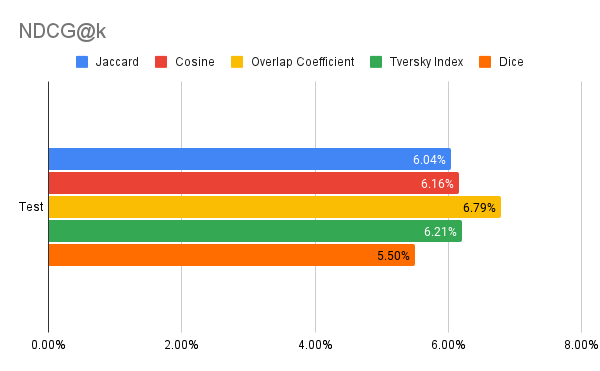
\includegraphics[width=3.5in]{picture/WR_MF-NDCG@k.png}
  For each similarity method, the chart values depict the percentage improvement achieved through the application of the respective 
  similarity measurement using WR-MF.
  \DeclareGraphicsExtensions.
  \caption{Improvement of NDCG score after application of the hybrid method}
  \label{fig:wrmf_ndcg}
\end{figure}

\begin{figure}[!t]
  \centering
  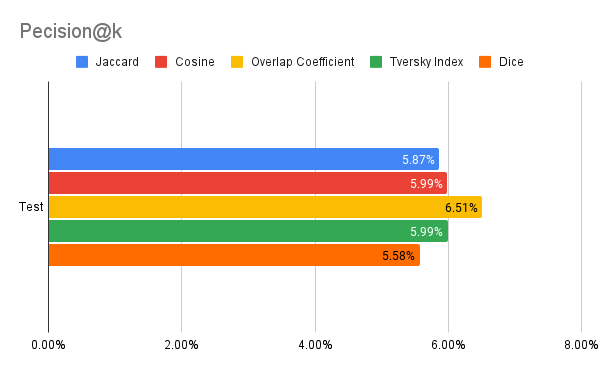
\includegraphics[width=3.5in]{picture/WR_MF-Pecision@k.png}
  For each similarity method, the chart values depict the percentage improvement achieved through the application of the respective 
  similarity measurement using WR-MF.
  \DeclareGraphicsExtensions.
  \caption{Improvement of precision after application of the hybrid method}
  \label{fig:wrmf_precision}
\end{figure}

\begin{figure}[!t]
  \centering
  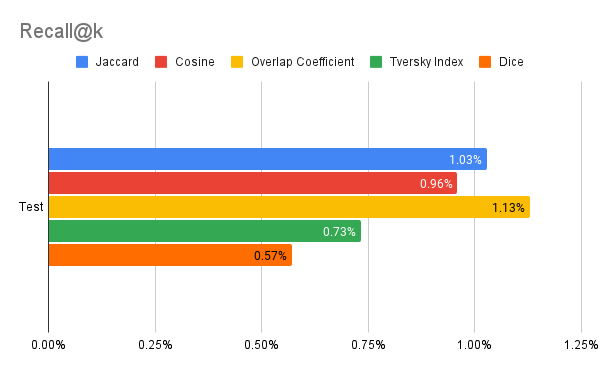
\includegraphics[width=3.5in]{picture/WR_MF-Recall@k.png}
  For each similarity method, the chart values depict the percentage improvement achieved through the application of the respective 
  similarity measurement using WR-MF.
  \DeclareGraphicsExtensions.
  \caption{Improvement of recall after application of the hybrid method}
  \label{fig:wrmf_recall}
\end{figure}

Applying the mentioned similarity measure to identify analogous items, the subsequent chart illustrates improvements observed in 
NDCG@k, Precision@k, and Recall@k on testing datasets. The utilization of this similarity measure has evidently resulted in 
enhanced predictive performance, as depicted by significant shifts in the mentioned evaluation metrics in Fig(\ref{fig:wrmf_ndcg}) 
, Fig(\ref{fig:wrmf_recall}), and Fig(\ref{fig:wrmf_precision}). As discerned from the observations, the Overlap coefficient and Cosine similarity measures outperform 
in accurately matching similar items within the hybrid implementation. Going beyond numerical scores, it is noteworthy that WR-MF 
exhibits a greater dependence on initial data for implicit prediction compared to BPR. Consequently, precision improves more 
significantly in WR-MF than in BPR.

% === VI. Dataset ========================
% =================================================================================
\section{Dataset}

\subsection*{Movie Lens 1M}
The ML-1M dataset was utilized to extract detailed information, encompassing rankings, movies, user profiles, and genre classifications. 
This dataset stands as a valuable resource, facilitating a comprehensive exploration and analysis of the intricate relationships and 
patterns within the realm of movies.

\subsection*{Movies and TV 5}
The amazon dataset for the movies was utilized to assess BPR ranking performance, this dataset does not cover the detailed information
about the movies, so the content extraction and similarity is not applicable for it.

% === VI. Conclusion ========================
% =================================================================================
\section{Conclusion}
In the realm of NDCG, the performance of both Bayesian Personalized Ranking (BPR) and Weight Regularized Matrix Factorization (WR-MF) 
stands remarkably similar. However, an innovative approach involving the integration of pre-processed similar ratings into the 
dataset reveals interesting nuances. This experimentation highlights that WR-MF demonstrates a heightened responsiveness to the 
newly introduced ratings, leading to a more substantial improvement compared to BPR.

While the comparative analysis underscores the enhanced sensitivity of WR-MF to the augmented dataset, it's important to consider 
the computational aspects. BPR, in contrast, exhibits a lower computational demand, suggesting a trade-off between sensitivity to 
new ratings and processing efficiency. This insight into their respective strengths and efficiencies adds valuable perspective to 
the evaluation of recommendation algorithms.

Based on the comprehensive iterations conducted with both WR-MF and BPR, the Overlap Coefficient emerges as the standout similarity 
measure. Through a thorough examination of their respective performances, the Overlap Coefficient consistently outshines other measures 
in capturing the similarity between items. This finding underscores the robustness and efficacy of the Overlap Coefficient in the 
context of recommendation systems, offering valuable insights for optimizing the similarity calculations in such algorithms.

\ifCLASSOPTIONcaptionsoff
  \newpage
\fi

\bibliographystyle{IEEEtran}
\bibliography{IEEEabrv,Bibliography}

\begin{IEEEbiographynophoto}{Mehdi Valinejad}
Received the B.S. degree in industrial engineering from the Azad University (South Tehran Branch) in 2012, and is currently working Master's. degree at the University of Bahcesehir at Istanbul.
\end{IEEEbiographynophoto}

\end{document}


